\documentclass[oneside,a4paper,english,links]{amca}
%
\usepackage{graphicx}
\usepackage{amsmath,amsfonts}
\usepackage{fullpage}
\usepackage{subfig}

% Shortcuts (should be in a separate file)
% Author comments 
\newcommand{\rodrigo}[1]{\authnote{Rodrigo}{#1}}

%% A simple dot to overcome graphicx limitations
\newcommand{\mydot}{.}

% TODO
\newcommand{\todo}[1]{\textbf{[TODO: #1]}}


\title{Bread Crumb classification using fractal and multifractal features}

\author[a]{Rodrigo Baravalle}
\author[b]{Claudio Delrieux}
\author[a]{Juan Carlos G\'omez}
%
\affil[a]{Laboratorio de Sistemas Din\'amicos y Procesamiento de Informaci\'on,
FCEIA, Universidad Nacional de Rosario\\ - CIFASIS - CONICET,
Riobamba 250 bis, 2000, Rosario, Argentina,
\{baravalle,gomez\}@cifasis-conicet.gov.ar, \url{http://www.fceia.unr.edu.ar/lsd/}}
%
\affil[b]{DIEC, Universidad Nacional del Sur - IIIE-CONICET,
Avenida Col\'on 80 - Bah\'ia Blanca(8000FTN) - Provincia de Buenos Aires - Rep\'ublica Argentina,
cad@uns.edu.ar, \url{http://www.ingelec.uns.edu.ar/}}

%% NOTE: IF ALL AUTHORS BELONG TO THE SAME AFFILIATION
%% USE THE `\voidaffil' MACRO FOR THE AFFILIATION CODE.
%% Example:
%% \author[\voidaffil]{First A. Author}
%% \author[\voidaffil]{Second B. Author}
%% \author[\voidaffil]{Third C. Author}
%% \author[\voidaffil]{Fourth D. Author}
%% %
%% \affil[\voidaffil]{Grupo de Mec\'anica Computacional,
%% Universidad Nacional de Villa Carolina,
%% Los Alerces 3492, 4200 Villa Carolina, Argentina,
%% gmc@uncarolina.edu.ar, http://www.uncarolina.edu.ar/gmc}

\begin{document}
\vspace{3cm}

\maketitle

%% To set PDF METADATA: uncomment and replace fields in
%% UPPERCASE with appropriate values. 
%% 
%% \hypersetup{
%%   pdfauthor={AUTHORS},
%%   pdfkeywords={KEYWORDS},
%%   pdftitle={TITLE}
%% }
%%
%% For instance
%% \hypersetup{
%%   pdfauthor={Sponge B. and Star P.},
%%   pdfkeywords={multiphase flow, air-liquid mixtures},
%%   pdftitle={A new model for multi-phase flow}
%% }
%%
%% NOTE: To set the metadata is recommended but not absolutely
%% neccesary. 
%% This was done before with the \pdfinfo command,
%% but according to this post:
%% http://de.nntp2http.com/comp/text/tex/2008/12/5358fd061de9703a781885a5dcf98364.html
%% if `hyperref' is used, then you must use \hypersetup{} not \pdfinfo{}

\begin{keywords}
Fractal, Multifractal, Classification, Bread crumb, Support Vector Machines
\end{keywords}

\begin{abstract}
Adequate image descriptors are fundamental in image classification and object recognition. For this purpose, it is required to identify image features that are both robust and of low dimensionality, in a way such that the classification process can be performed in a variety of situations and with a reasonable computational cost. 

In this context, the identification of materials posses a significant challenge, since usual (geometric and/or differential) feature extraction methods are not robust enough. Texture features based on Fourier or wavelet theories, on the other hand, do withstand geometric and illumination variations, but tend to require a high amount of descriptors to perform adequately. 

Recently, the theory of fractal sets has shown to provide local image features that are both robust and low-dimensional. In this work we apply fractal and multifractal feature extraction for bread crumb classification based on color scans of slices of different bread types. Preliminary results show that fractal based classification is able distinguish different bread
crumbs with very high accuracy.
\end{abstract}

\section{Introduction}
Fractal and multifractal analysis of images have demonstrated to capture useful properties of the underlying material represented. Characterisation of images using these features have been successfully applied in different fields, for instance medicine \cite{Andjelkovic2008,Yu2011} and texture classification \cite{Wendt2009}. Through several procedures, it is possible to obtain differents Fractal Dimensions (FD), each of them capturing a different property of the material (e.g., void fraction, rugosity).

For each material, the results obtained in the classification process are useful in quality measurements of real samples and also in the validation of synthetic representations of them. In other words, the classification is useful to determine if a given image presents the observed features in that material, permitting to establish quality parameters to them. In~\cite{Fan2006}, a quality bread crumb test was performed, obtaining similar results. Nevertheless, a smaller database was used ($30$ images). In \cite{Gonzales2008} several fractal features were obtained for one type of bread, showing that a vector comprising them would be capable of represent its crumb texture.

In this work we propose the application of fractal and multifractal descriptors to classify among different bread types and to discriminate between bread and non-bread images. The proposed method is compared to a classifier that uses only mean color information. The results of this feature extraction procedure are shown to be both robust and simple to discriminate bread images from non bread ones. In section $2$ we briefly introduce the theory underlying fractal sets. In section $3$ we describe the materials and methods employed in the classification. In section $4$ we show the results obtained in the classification and we perform a robustness analysis of the method. In section 5 we summarise the conclusions, and we pose some possible future works.

\section{Features}
\subsection{Box Dimension}
Box FD is a simplification of the Hausdorff (originaly Minkowski - Bouligand) dimension for non strictly self-similar objects \cite{Peitgen2004}. Given a binarised image, it is subdivided in a grid of size $M\times M$ where the side of each box formed is $\epsilon$. If $N_{\epsilon}$ represents the amount of boxes that contains at least one pixel in the binarisation of the set for that $\epsilon$, then the computation of the box dimension  $D_{b}$ is as shown in Eq. (\ref{eqn:eqn1}).

\begin{equation}
D_{b} = \displaystyle\lim_{\epsilon \to 0}{\frac{\log(N_{\epsilon})}{\log (1/\epsilon)}}.
\label{eqn:eqn1}
\end{equation}

The algorithm computes a binarised image of the original and then selects differents $\epsilon$ in it, making a count of the boxes that contains pixels in each case (to avoid numerical instabilities, a mean of cases is computed, establishing differents positions in the grid over the image). Finally, a linear regression adjustment is made with the obtained data, in the $\log-\log$ space, and the slope of the data is by definition the box dimension of the image. In Fig. \ref{fig:fitbox} an image of the bread type {\em salvado} is shown with its box dimension computation.

\begin{figure*}[htb]
\centering
$\vcenter{\hbox{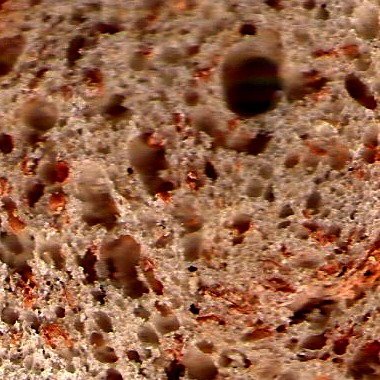
\includegraphics[scale=1.3]{imagenes/salvado19}}}$
$\vcenter{\hbox{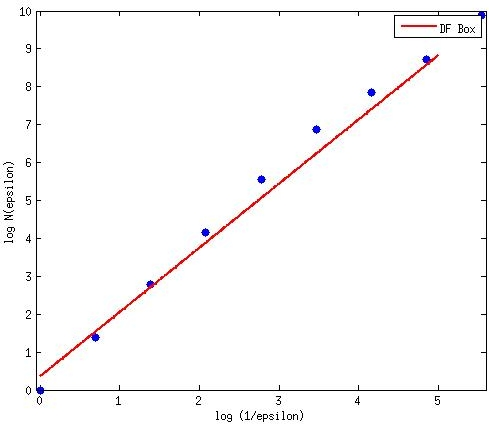
\includegraphics[scale = 0.4]{imagenes/fitbox}}}$
\caption{An image and its box dimension computed}
\label{fig:fitbox}
\end{figure*}

\subsection{Morphological Fractal}
This FD is computed through dilation and erosion operations, using a structuring element (SE). The transformed image is function of the distribution of that particular SE in the original image.  In this case, the SE is a rhombus $Y$ with scales that varies from $\epsilon = 1$ to $\epsilon = 7$ (and the areas of the SE between $5$ and $113$ pixels)  . The surface area can be calculated, for each $\epsilon$ as in Eq. (\ref{eqn:eqn2}) \cite{Gonzales2008}.

\begin{equation}
S(X,Y,\epsilon) = \frac{\sum_{x,y \in M} (f_{\epsilon}^{u}(x,y) - f_{\epsilon}^{l}(x,y))}{2\epsilon}.
\label{eqn:eqn2}
\end{equation}

$f_{\epsilon}^{u}(x,y)$ is the $\epsilon$-th dilation and $f_{\epsilon}^{l}(x,y)$ is the $\epsilon$-th erosion of the original image. The morphological FD $M_{d}$ is estimated from the slope of a linear regression adjustment of the data in $S(X,Y,\epsilon)$ and $\epsilon$ in the $\log-\log$ space.

\begin{equation}
M_{d} = 2 + m.
\label{eqn:eqn3}
\end{equation}

\subsection{Multifractal Analysis}
Some elements in nature show fractal features or autosimilarity. The fractal dimension is an exponent which relates the statistical autosimilarity of the object at different scales. On the one hand, deterministic fractals are characterized by the same FD at all scales. They are called {\em monofractals} (for instance, Koch Curve, Sierpinsky triangle). On the other hand, {\em multifractals} \cite{Mandelbrot89} are characterized by a set of FDs depending on the scale. It is assumed that these structures are composed by different fractals coexisting simultaneoulsy. In a previous work \cite{Baravalle2012}, it has been shown, using the Box Dimension and the Korcak Dimension \cite{Imre11}, that the object of study of this work presented multifractal features. As a consequence, fractal and multifractal features are taken into account.

\subsubsection*{H\"older Exponent}
Informally, the way to proceed with multifractal analysis is to examine, in the limit, the local behaviour of a measure $\mu$ at each point of the set in study. This means, to find the H\"older exponent $\alpha$ in that point. The {\em multifractal spectrum} $f(\alpha)$ is obtained applying this procedure to the entire set, in this case, an image.

Let $E$ be an structure divided in substructures $E_{i}$ of size $\epsilon$ in such a way that $U_{i}E_{i} = E$. Each substructure $E_{i}$ is characterized by a measure $\mu(E_{i})$. From the point of view of multifractal analysis, it is useful to define this value as a function of $\epsilon$.


\begin{equation}
\alpha_{i} = \frac{ln(\mu(E_{i}))}{ln(\epsilon)},
\label{eqn:eqn4}
\end{equation}

and to take the limit when $\epsilon$ tends to $0$. The limit represents the value of the H\"older exponent at a point in the structure.

\begin{equation}
\alpha = \lim_{\epsilon\to0}{\alpha_{i}},
\label{eqn:eqn5}
\end{equation}

The exponent characterizes the local regularity of the structure at a point. To obtain a global characterization of its regularity it is needed to obtain the distribution of $\alpha$ in $E$. For this, a count must be done for each $\alpha_{i}$, related to the value of $\epsilon$ (Eqn. \ref{eqn:eqn6}).

\begin{equation}
f_{\epsilon}(\alpha_{i}) = - \frac{ln(N_{\epsilon}(\alpha_{i}))}{ln(\epsilon)},
\label{eqn:eqn6}
\end{equation}

When $\epsilon$ tends to $0$, the limiting value is the FD of the structure $E$ characterized by $\alpha$, the Hausdorff dimension of the $\alpha$ distribution, also known as the {\em multifractal spectrum} $f(\alpha)$ \cite{Silvetti2010} (Eq. \ref{eqn:eqn7})

\begin{equation}
f(\alpha) = \lim_{\epsilon\to0}{f_{\epsilon}(\alpha)}.
\label{eqn:eqn7}
\end{equation}

\subsubsection*{Procedure}
To obtain the H\"older exponent at a given pixel, a linear regression adjustment is needed using the values ($log(\epsilon)$,$log(\mu(E_{i})$), for $\epsilon = 2i + 1, i \ge 0$, where $E_{i}$ are boxes of length $\epsilon$ centered at the pixel. The slope of the adjustment is the desired H\"older exponent.

From the $\alpha$ values a new image is generated in grey scale ($\alpha$ image), with the same dimensions of the original, where the value at each pixel is a mapping from the exponent to that scale. Since it is possible to obtain $M\times M$ values per image (where $M\times M$ is the dimension in pixels of the image), it is necessary to define a number $C$ of classes (the number could be a parameter), each of which establish $\alpha$ range values, and calculate the spectrum only for those values.

Let $\alpha_{min}$ and  $\alpha_{max}$ be the minimum and maximum values of $\alpha$ computed in the image. $C$ values are defined $\alpha_{c} = \alpha_{min} + (c-1)(\alpha_{max}-\alpha_{min})/C$, where $c = 1,2,\dots,C$. Then, $\alpha \in \alpha_{c}$ if $\alpha_{c} \leq \alpha < \alpha_{c+1}$. If $\alpha = \alpha_{max}$, then $\alpha \in \alpha_{C}$. Finally, a linear regression adjustment is obtained for the values $N_{\epsilon}(\alpha)$ and $\epsilon$ in the $\log-\log$ space. The value of the slope is the FD $f(\alpha_{c})$ and must be calculated for $c = 1,2,\dots,C$. In this way $C$ $f(\alpha)$ values are obtained, representing $C$ FDs ($C$ $\alpha_{c}$ associated values are also obtained). In this work all these values are used as features in order to do the classification (so $2\times C$ features are obtained from the multifractal analysis). In Fig. \ref{fig:emf} an image of lactal bread and its multifractal analysis are shown (in this case, $C = 20$).

\begin{figure*}[htb]
\centering
$\vcenter{\hbox{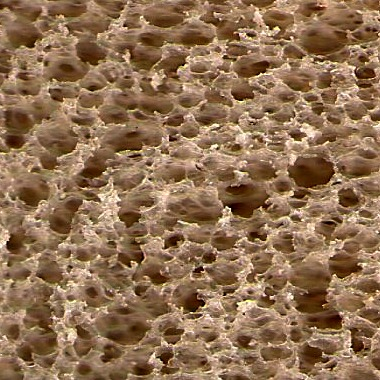
\includegraphics[scale=1.3]{imagenes/lactal31}}}$
$\vcenter{\hbox{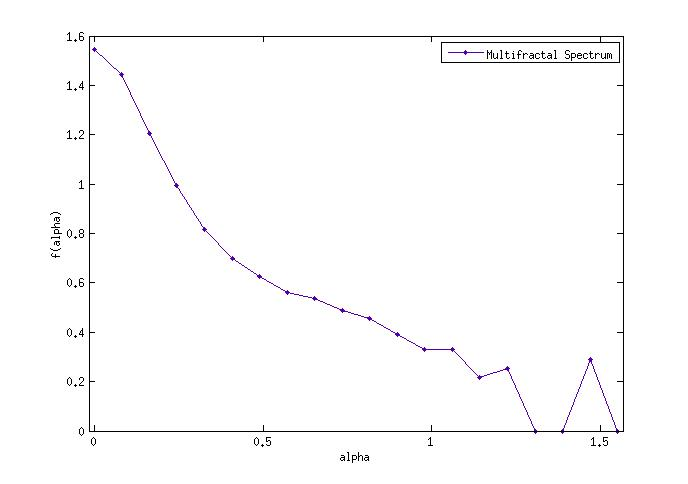
\includegraphics[scale = 0.4]{imagenes/emf}}}$
\caption{Image and its multifractal spectrum (20 FDs)}
\label{fig:emf}
\end{figure*}

\section{Materials and Methodology}

\subsection{Image Acquisition}
Fifty images of four different bread types (lactal, baguette, salvado and sandwich), counting two hundred ($200$) images, were obtained using an electric slicer (in the case of baguette and salvado, since the two other types were already sliced in the moment of purchase). The images were digitalised using an HP PSC 1210 scanner and they were saved in TIFF format. Images showed a resolution of $380 \times 380$ pixels (the maximum possible surface for the four types of bread) and $350$ dpi ($1$ pixel - $0.00527 mm^{2}$). Then they were converted to grey scale ($8$ bits). Also $20$ images of each bread type were taken with a digital camera, using the same spatial resolution, counting $80$ images. The illumination conditions of these images were different from that of the scanner in order to test for the robustness of the method. In Fig. \ref{fig:camera} four examples of bread images from the camera are shown. We also employed 20 \todo{Check} randomly selected images from the CalTech101~\cite{FeiFei04} dataset in order to test the method's performance with non-bread images. In Fig.~\ref{fig:nonbread} four examples of non-bread images from this dataset are shown. 

In those cases where the utilised procedure uses a binarisation of the original image, it was obtained using the White's algotithm \cite{White83}. This algorithm applies a local thresholding schema, which showed better results in comparison to those obtained using a global thresholding schema. Particularly, the algorithm presented in \cite{Huang95} and used in \cite{Gonzales2008}, showed poor results when the illumination conditions varies. Since the center of air bubbles with bigger areas appeared as black pixels, instead of white (and since those areas are characterized as dark regions in the original image), a global grey threshold using Otsu's algorithm \cite{Otsu79} is obtained and multiplied with a scalar which is a parameter, setting as white the resulting pixels in the final binarisation. It was found that defining the scalar as $0.8$ showed acceptable results. So the combination of local and global thresholding makes it an hybrid algorithm. In Fig.~\ref{fig:bread} an image of each bread type used in this work and its resulting binarisaton using the proposed algorithm is shown.  


\begin{figure*}[htb]
\centering
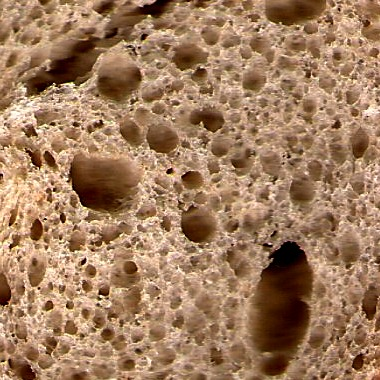
\includegraphics[scale=1.3]{imagenes/baguette20}
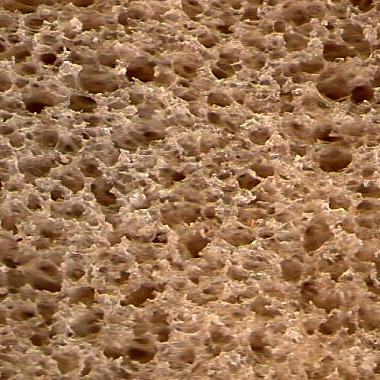
\includegraphics[scale=1.3]{imagenes/lactal14}
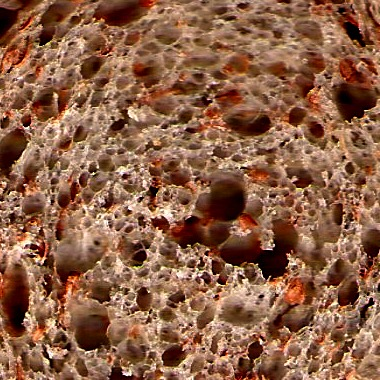
\includegraphics[scale=1.3]{imagenes/salvado43}
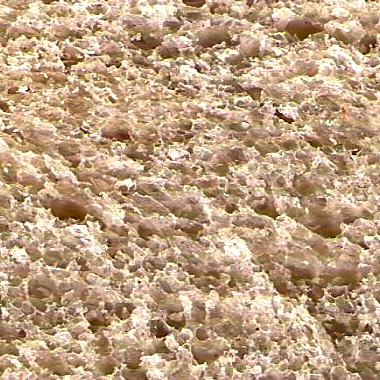
\includegraphics[scale=1.3]{imagenes/sandwich43}
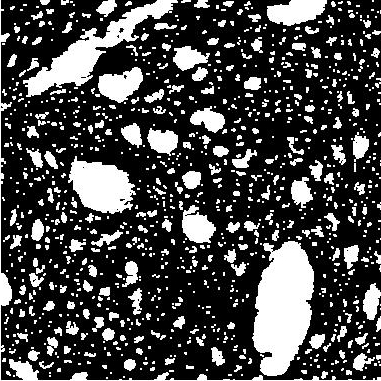
\includegraphics[scale=0.265]{imagenes/baguette20bin}
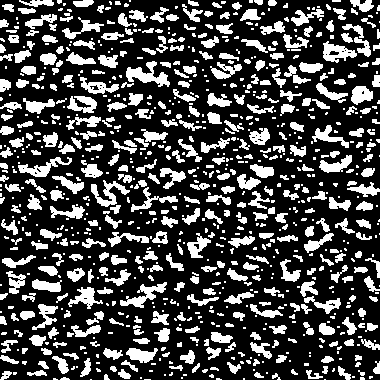
\includegraphics[scale=0.333]{imagenes/lactal14bin}
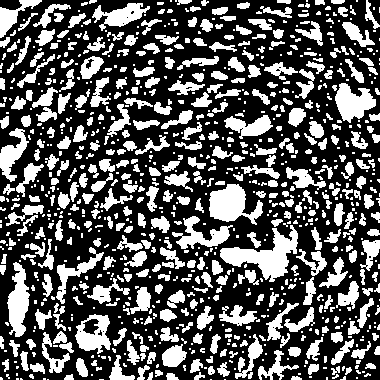
\includegraphics[scale=0.333]{imagenes/salvado43bin}
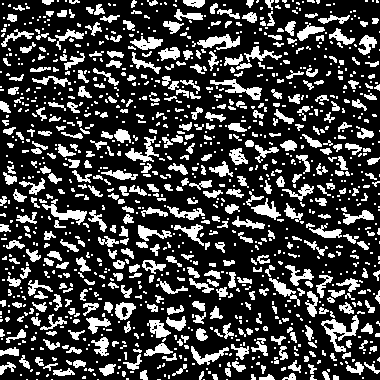
\includegraphics[scale=0.333]{imagenes/sandwich43bin}
\caption{Digitalised images of Baguette, Lactal, Salvado and Sandwich bread types with its binarisations}
\label{fig:bread}
\end{figure*}

\begin{figure*}[htb]
\centering
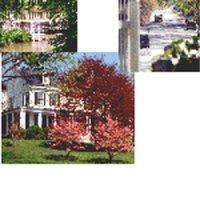
\includegraphics[scale=0.5]{exps/100sample/image_0004}
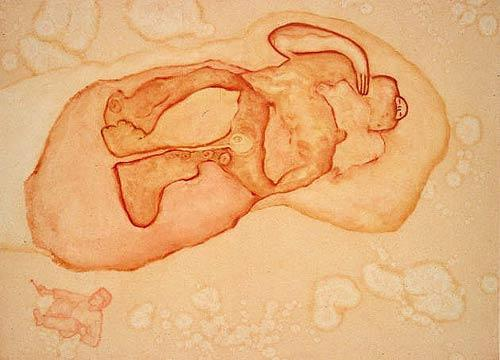
\includegraphics[scale=0.2]{exps/100sample/image_0019}
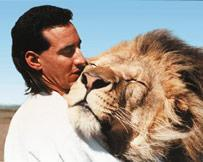
\includegraphics[scale=0.5]{exps/100sample/image_0027}
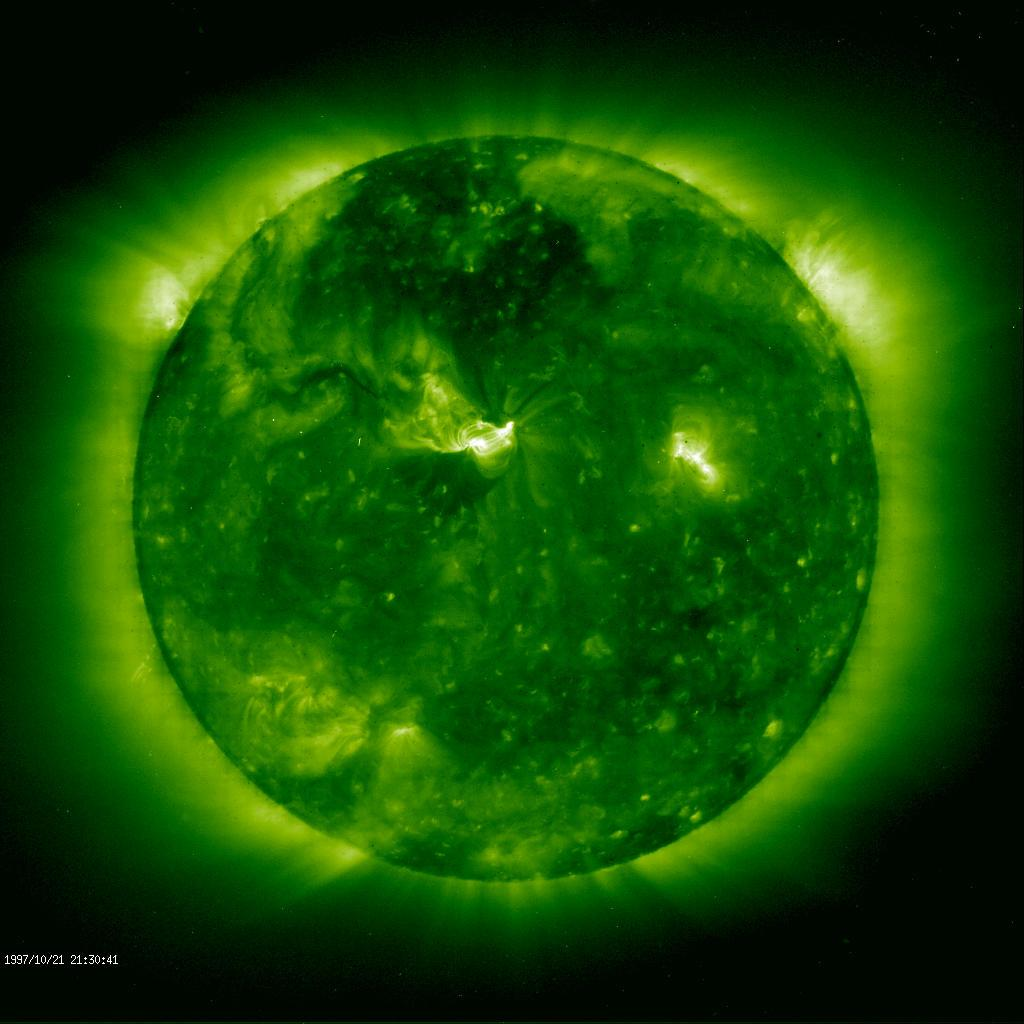
\includegraphics[scale=0.1]{exps/100sample/image_0309}
\caption{Images from the dataset CalTech101}
\label{fig:nonbread}
\end{figure*}

\begin{figure*}[htb]
\centering
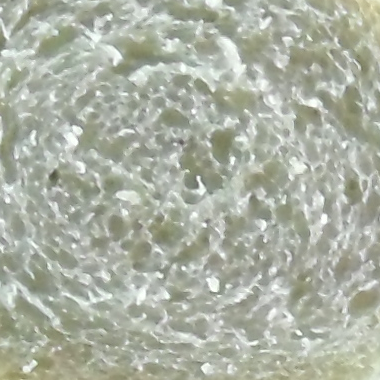
\includegraphics[scale=0.28]{imagenes/camera/b}
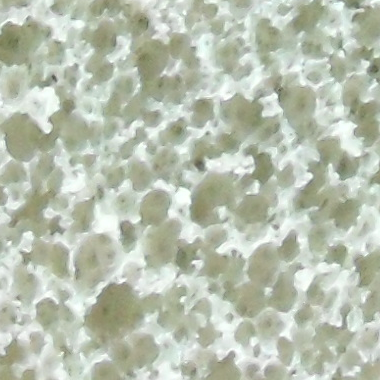
\includegraphics[scale=0.28]{imagenes/camera/l19}
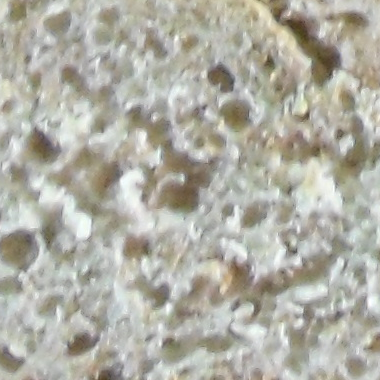
\includegraphics[scale=0.28]{imagenes/camera/s7}
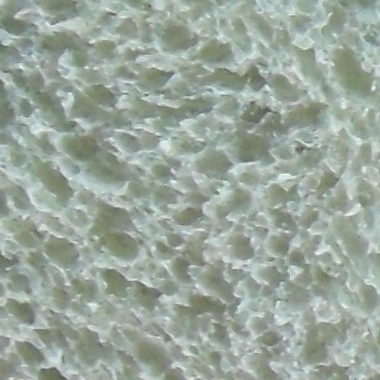
\includegraphics[scale=0.28]{imagenes/camera/Sa14}
\caption{Digitalised images from a digital camera}
\label{fig:camera}
\end{figure*}

\subsection{Feature Vectors}


Following the ideas presented in \cite{Gonzales2008}, the mentioned fractal and multifractal features were obtained for each image (using $20$ H\"older exponents). For each image, a $42$ features vector was computed. The code of the algorithms Box dimension, Morphological fractal dimension and the multifractal spectrum was written and run in Matlab. In order to make a comparison, a vector with RGB color features was computed (R mean, G mean, B mean) in a $3$ dimension features vector.

A self-organizing maps (SOM)~\cite{Kohonen2001} of the vectorized images are useful to visualize these different representation of bread images into a lower dimensional view, in order to understand them better. A SOM maps high dimensional data into a (tipically) two-dimensional representation, using neighborhood information. Topological information of the original data is preserved.  

An unsupervised SOM of the fractal and non fractal representation of scanned images are shown in Fig.~\ref{fig:somfractal} and Fig.~\ref{fig:somrgb} respectively. The fractal features SOM seems to show easily separable classes and the RGB features SOM appears to be more overlapped. Also, in the latter, the non bread class seems to be spread over the rest of the classes, making it more difficult to distinguish between bread and non bread types. It seems that a classificator could potentialy obtain better classification results using the fractal features. %%Next sections will show that this hypothesis is true.

\begin{figure*}

\begin{centering}
\subfloat[Fractal features SOM]{\begin{centering}
\includegraphics[width=0.6\textwidth]{exps/som/som\mydot multifractal}
\label{fig:somfractal}
\par\end{centering}
}
\par\end{centering}

\begin{centering}
\subfloat[SOM using RGB features]{\begin{centering}
\includegraphics[width=0.6\textwidth]{exps/som/som\mydot rgb}
\label{fig:somrgb}
\par\end{centering}
}
\par\end{centering}

\caption{SOM of the scanned bread images (classes $1$~--~$4$) and the non bread images (class $5$)}

\end{figure*}

%\begin{figure*}[]
%\centering
%\includegraphics[width=0.55\textwidth]{exps/som/som\mydot multifractal}
%\caption{Self organizing maps for the Fractal features: $1 =$ baguette,$2 =$ lactal, $3 =$ salvado, $4 =$ sandwich, $5 =$ non bread }
%\label{fig:somfractal}
%\end{figure*}

%\begin{figure*}[]
%\centering
%\includegraphics[width=0.55\textwidth]{exps/som/som\mydot rgb}
%\caption{Self organizing maps for the non Fractal features}
%\label{fig:somrgb}
%\end{figure*}

\section{Results}

\subsection{Classification}
{\em Support Vector Machines} (SVM)~\cite{Boser92} were utilised to perform the classification, using {\em libsvm}~\cite{Chang2011} implementation.
%\subsection{Scanned Images}
The method {\em k-fold cross validation} was utilised in order to validate the results with $k = 4$, i.e., $75\%$ of samples are used as training and $25\%$ as test (then switching the training and test samples). Table \ref{table:tableFirstTest} shows classification results for both methods of classification, using $50$ scanned images of each type (i.e. $250$ images, including $50$ of non bread images). It can be seen that the utilisation of non-fractal features in the images gives comparable results to that of using fractals features.

\begin{table}[htb]
\centering
\begin{tabular}{|c|c|c|}
    \hline
    Features & Fractals & non Fractals\\
    \hline
    Accuracy  & $\textbf{88.4}\%$ & $86\%$\\
    \hline
\end{tabular}
\caption{Results obtained in classification}
\label{table:tableFirstTest}
\end{table}

\subsection{Robustness Test}
In order to test for the robustness of the method, $20$ scanned images from each class, and $20$ from the CalTech101 dataset, were used as train and all the images from the digital camera ($20$ per class), and $20$ non bread images were used as test (counting $100$ images). In Table \ref{table:tableRobustness} accuracy results of both methods are shown. Results shows poor performance of both classifiers. Nevertheless, in Tables \ref{table:ConfusionMatrixFractal} and \ref{table:ConfusionMatrixNonFractal}, the confusion matrix of the data using both methods is shown. It can be seen that the RGB method assigns all the data to the non bread class, while the fractal features are able to discriminate between images of breads and non breads, making it a good discriminator of non bread images.

\begin{table}[htb]
\centering
\begin{tabular}{|c|c|c|}
    \hline
    Features & Fractals & non Fractals\\
    \hline
    Accuracy  & $\textbf{40}\%$ & $20\%$\\
    \hline
\end{tabular}
\caption{Results obtained in classification}
\label{table:tableRobustness}
\end{table}


\begin{table}[htb]
\centering
\begin{tabular}{|c|c|c|c|c|c|}
    \hline
    Classes & Baguette & Lactal & Salvado & Sandwich & Non bread\\
    \hline
    Baguette    &   $0$  &   $9$  &   $0$  &  $11$ &   $0$\\
    \hline
    Lactal  & $0$ & $15$ & $0$ & $5$ & $0$\\
    \hline
    Salvado & $0$ & $6$ & $0$ & $12$ & $2$\\
    \hline
    Sandwich  & $0$ & $10$ & $0$ & $10$ & $0$\\
    \hline
    Non bread  & $3$ & $0$ & $2$ & $0$ & $15$\\
    \hline
\end{tabular}
\caption{Confusion Matrix for the fractal features}
\label{table:ConfusionMatrixFractal}
\end{table}

\begin{table}[htb]
\centering
\begin{tabular}{|c|c|c|c|c|c|}
    \hline
    Classes & Baguette & Lactal & Salvado & Sandwich & Non bread\\
    \hline
    Baguette  & $0$ & $0$ & $0$ & $0$ & $20$\\
    \hline
    Lactal  & $0$ & $0$ & $0$ & $0$ & $20$\\
    \hline
    Salvado & $0$ & $0$ & $0$ & $0$ & $20$\\
    \hline
    Sandwich  & $0$ & $0$ & $0$ & $0$ & $20$\\
    \hline
    Non bread  & $0$ & $0$ & $0$ & $0$ & $20$\\
    \hline
\end{tabular}
\caption{Confusion Matrix for the RGB features}
\label{table:ConfusionMatrixNonFractal}
\end{table}

\subsection{Deceiving the classifier}
It is possible to mislead the classifiers with false images. Fig. \ref{fig:fakeRGB} shows an image that is classified as bread by its RGB features. Fig. \ref{fig:fakeMultifractal} shows an image generated by a particle system~\cite{Baravalle2011} which is classified as bread by its multifractal features. It is easy to deceive the RGB classifier, using images with similar color features as breads, but it is not clear how to do that with fractal features. We conclude that the fractal classifier is more accurate to discriminate these false images.

\begin{figure*}[]
\centering
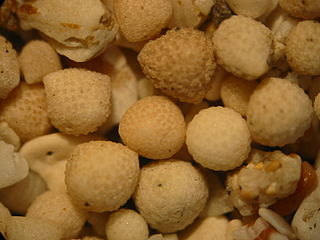
\includegraphics[width=0.45\textwidth]{exps/fake/320px-Sand_from_Kuta,_Bali,_Indonesia}
\caption{A non bread image classified as bread by its RGB featues}
\label{fig:fakeRGB}
\end{figure*}

\begin{figure*}[]
\centering
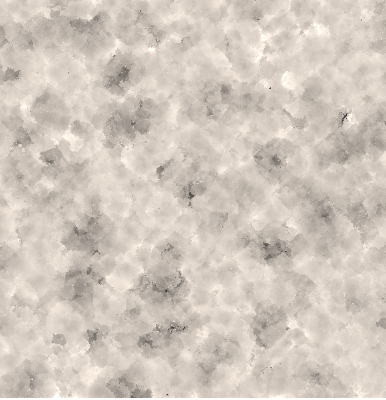
\includegraphics[width=0.25\textwidth]{exps/fake/6}
\caption{A synthetic image is classified as bread by its fractal features}
\label{fig:fakeMultifractal}
\end{figure*}

%\subsection{Variable Selection}
%\todo{Add PCA explanation and results} \\
%\todo{Add PCA float table in a minipage next to the table1}

\section{Conclusions and Future Work}
The utilisation of fractal and multifractal features in bread crumb texture classification showed good performance. The multifractal spectrum demonstrated to be accurate enough to perform a classification of differents bread types and also to discriminate non bread from bread images. The utilisation of non-fractal features such as color, also showed comparable results, but it fails to detect non bread images, and it is easy to deceive it with false images. Both methods showed to be sensitive to illumination changes, making the method still non robust. Preliminary tests on our particle system~\cite{Baravalle2011}  show that it could deceive the fractal classifier, so further analysis is required.

The results found can be applied to validate synthetic samples, i.e., the latter should have similar features to certain bread type that it is trying to simulate. The features obtained will be used to determine particle system parameters (e.g., lifetime of particles, color). These results can be extended to be used as quality parameters for these products. The robustness of the method needs to be enhanced, the utilisation of other types of DFs to accomplish it will be studied. The code of the multifractal spectrum algorithm is unoptimized, so an optimisation needs to be applied.

%
\bibliography{bibliografia/amcapaper}
\end{document}
% $Id: amcapaper.tex,v 1.23 2006/08/14 16:58:45 mstorti Exp $
